\section{Half-precision floating-point numbers}





\begin{figure}[H]
    \centering
    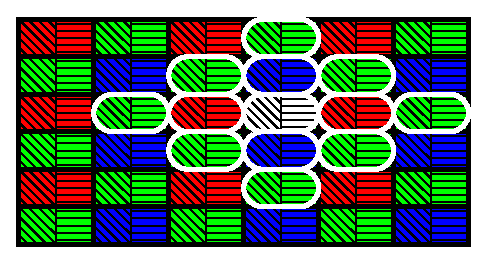
\includegraphics[width=0.45\textwidth]{figures/polarized_image/half2_conv.pdf}
    \caption{TODO}
    \label{fig:}
\end{figure}

\subsection{Small Infinities}

Half-precision floating points consider any value exceeding $65504$ as infinity \cite{HalfprecisionFloatingpointFormat2023}. This can pose a problem when performing calculations that might exceed this threshold during intermediate steps, resulting in the value being treated as infinity. In the preprocessing phase, this issue occasionally arises since the \code{P010_10LE} format utilizes the 10 most significant bits of a 16-bit integer, approaching the limit of half-precision floating points.

This was particularly problematic when the resulting values were cast to integers, as the resulting value would be zero, causing unexpected black spots in the image.
To mitigate this problem, the floating-point values are now cast to integers within the range of 0 to 1023, followed by a left bitshift of 6 bits to conform to the \code{P010_10LE} format.


